\documentclass{beamer}
\usepackage{graphicx}
\usepackage[utf8]{inputenc}
\usepackage{verbatim}
\setlength{\parindent}{0pt}
\setlength{\parskip}{10pt plus 6pt minus 4pt}

\usetheme{UTBM}
%\usecolortheme{UTBM}

\begin{document}

\begin{frame}
\frametitle{Handover}
\begin{center}
  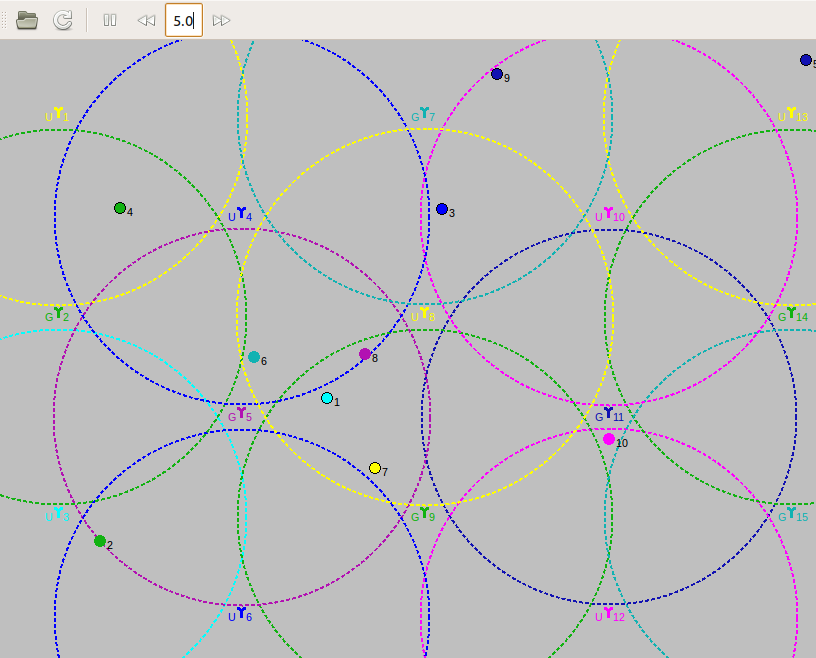
\includegraphics[width=0.6\textwidth]{./images/capture.png}
\end{center}

Mathieu BRIAND \\
Marine JOURDAIN

\end{frame}

%%%%%%%%%%%%%%%%%%%%%%%%%%%%%%%%%%%%%%%%%%%%%%%%%%%%%%%%%%%%%%%%%%%%%%%%%%%%%%%

\begin{frame}
\frametitle{Plan}
\tableofcontents

\end{frame}

%%%%%%%%%%%%%%%%%%%%%%%%%%%%%%%%%%%%%%%%%%%%%%%%%%%%%%%%%%%%%%%%%%%%%%%%%%%%%%%
\section{Subject}

\begin{frame}
\frametitle{Subject}
Inputs for each BTS :
\begin{itemize}
  \item Pe : Emission power
  \item Ge : Emission gain
  \item F : Frequency
  \item HO\_MARGIN : Minimum marge between two signals to allow handover ;
  \item MS\_TXPWR\_MAX : Maximum emission power allowed to be used by the MS in a cell.
\end{itemize}

\end{frame}
%%%%%%%%%
\begin{frame}
\begin{itemize}
  \item BTS\_TXPWR\_MAX : Maximum emission power allowed to be used by the BTS in a cell.
  \item RXLEV\_MIN : Electromagnetic field level to access to a cell.
  \item MAX\_MS\_RANGE : Maximum distance between Mobile Station and BTS.
  \item L\_RXQUAL\_H: Minimum quality to allow handover.
  \item L\_RXLEV\_DL\_H : Minimum received level to allow handover on downlink.
  \item L\_RXLEV\_UP\_H : Minimum received level to allow handover on uplink.
\end{itemize}
%%%%%%%%%%%%%
\end{frame}
%%%%%%%%%%%%%
\begin{frame}
Inputs for each Mobile Station (MS) :
\begin{itemize}
  \item Pe : Emission power
  \item Ge : Emission gain
  \item P : Maximum Emission Power of the MS
\end{itemize}

\end{frame}
%%%%%%%%%
\begin{frame}
Outputs\\

\begin{itemize}
    \item Log file
    \item Graphic interface with MS colored in the BTS color it is linked
(Python language)
      \begin{center}
        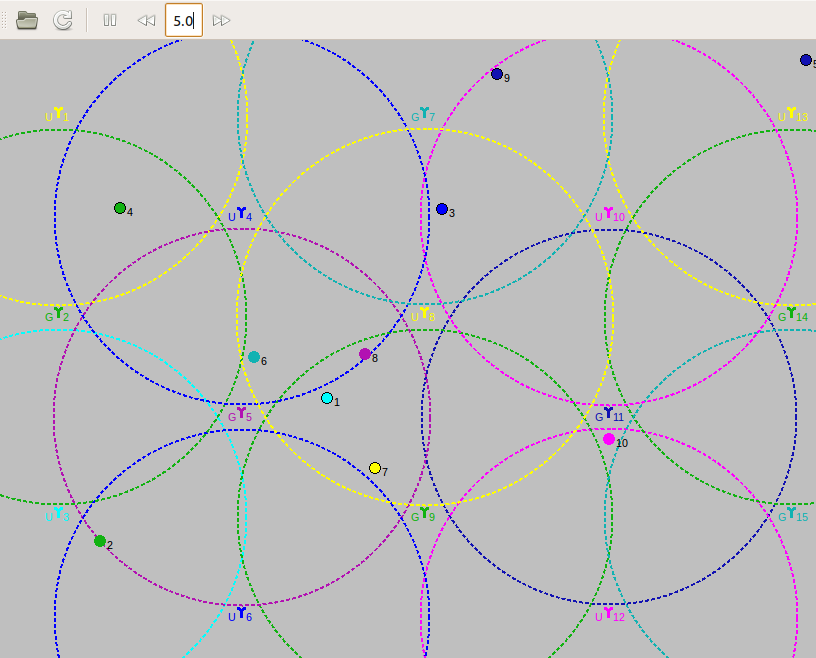
\includegraphics[width=0.4\textwidth]{./images/capture.png}
      \end{center}
\end{itemize}

\end{frame}

%%%%%%%%%%%%%%%%%%%%%%%%%%%%%%%%%%%%%%%%%%%%%%%%%%%%%%%%%%%%%%%%%%%%%%%%%%%%%%%
\section{Handover algorithm}

\begin{frame}
\frametitle{Handover algorithm}
\begin{itemize}
  \item Measure phase : RxLev uplink and downlink, RxQual uplink and downlink, Distances between MS and BTS each 40ms
  \item Mean phase on 12 samples each 480ms
  \item Storing between 8 and 12 means
  \item Construct neighbour list, looking measures of other cells
  \item For each cell of the neighbour list, decide if handover is possible.
  \item If handover is possible, the order to change of bts must be repeated 3
times.
\end{itemize}
\end{frame}
%%%%%%%%%%%%%%%%%%%%%%%%%%%%%%%%%%%%%%%%%%%%%%%%%%%%%%%%%%%%%%%%%%%%%%%%%%%%%%%
\section{Log file}

\begin{frame}[fragile]
\frametitle{Log file}

{\tiny
\begin{verbatim}
==============================
MS  1 , measure phase
current bts : 1
rxlev_dl_mean :  -63.8128912153
rxlev_up_mean :  -68.3553163097
rxqual_dl_mean :  7
rxqual_up_mean :  7
distanceMsBts_mean[ 5 ] :  43826.9506126
distanceMsBts_mean[ 1 ] :  10695.029425
distanceMsBts_mean[ 6 ] :  25929.6629448
distanceMsBts_mean[ 2 ] :  28140.8052454
distanceMsBts_mean[ 7 ] :  42148.589561
distanceMsBts_mean[ 4 ] :  49482.4074797
distanceMsBts_mean[ 3 ] :  30344.1517983
distanceMsBts_mean[ 8 ] :  52724.3006395
rxlev_ncell_mean[ 5 ] :  -79.7852334443
rxlev_ncell_mean[ 1 ] :  -70.461660669
rxlev_ncell_mean[ 6 ] :  -80.8401844516
rxlev_ncell_mean[ 2 ] :  -81.9337942304
rxlev_ncell_mean[ 7 ] :  -85.7305755869
rxlev_ncell_mean[ 4 ] :  -87.2517138375
rxlev_ncell_mean[ 3 ] :  -82.6400788618
rxlev_ncell_mean[ 8 ] :  -87.7114210819
neighbour_list : [ 1: 66.3512305463 ]
==============================
\end{verbatim}
}

\end{frame}

%%%%%%%%%%%%%%%%%%%%%%%%%%%%%%%%%%%%%%%%%%%%%%%%%%%%%%%%%%%%%%%%%%%%%%%%%%%%%%%
\begin{frame}[fragile]
\frametitle{Log file}

{\tiny
\begin{verbatim}
MS  3 , measure phase
current bts : 2
rxlev_dl_mean :  -62.3445170661
rxlev_up_mean :  -66.8869421605
rxqual_dl_mean :  7
rxqual_up_mean :  7
distanceMsBts_mean[ 5 ] :  16911.5936564
distanceMsBts_mean[ 1 ] :  27359.9064007
distanceMsBts_mean[ 6 ] :  38161.7981747
distanceMsBts_mean[ 2 ] :  9348.19654032
distanceMsBts_mean[ 7 ] :  35932.4628666
distanceMsBts_mean[ 4 ] :  18305.1916093
distanceMsBts_mean[ 3 ] :  18703.1507596
rxlev_ncell_mean[ 5 ] :  -71.4958167077
rxlev_ncell_mean[ 1 ] :  -80.6370179543
rxlev_ncell_mean[ 6 ] :  -84.408623444
rxlev_ncell_mean[ 2 ] :  -69.3785690197
rxlev_ncell_mean[ 7 ] :  -83.2518938146
rxlev_ncell_mean[ 4 ] :  -78.2988807803
rxlev_ncell_mean[ 3 ] :  -77.3825558191
neighbour_list : [ 2: 65.9659480463, 5: 63.8487003584 ]
rxlev_up_mean < l_rxlev_up_h :  12 / 10
rxlev_dl_mean < l_rxlev_dl_h :  12 / 10
rxqual_up_mean > l_rxqual_h :  7  / 6
rxqual_dl_mean > l_rxqual_h : 7  / 6
ho margin : 5
distance with BTS > max_ms_range : 10 / 8
pgbt > ho matgin : True
distance with BTS > max_ms_range : 10 / 8
pgbt > ho margin : True
MS 3 found new BTS 5 for possible handover
==============================
\end{verbatim}
}
\end{frame}
%%%%%%%%%%%%%%%%%%%%%%%%%%%
\begin{frame}[fragile]
\frametitle{Log File}

{\tiny
\begin{verbatim}
MS 7 asked for BTS 5 2 times
==============================

MS 3  handover from BTS 2 to BTS 5
==============================

\end{verbatim}
}

\end{frame}
%%%%%%%%%%%%%%
\begin{frame}
\frametitle{Study of parameters effects}
Creation of 4 configuration files, representing maps with BTS and 10 MS.
\begin{itemize}
 \item Overlap between BTS
 \item Handover margin
 \item Number of orders to change from a BTS to another
\end{itemize}
\end{frame}
%%%%%%%%%%%%%%%%%%%%%%%%%%%%%%%%%%%%%%%%%%%%%%%%%%%%%%%%%%%%%%%%%%%%%%%%%%%%%%%
\begin{frame}
\frametitle{Study of parameters effects}
For 1 order to change of BTS
\begin{itemize}
 \item High overlap and weak ho margin
  \begin{itemize}
    \item In a 5 min interval : 1874 handovers
  \end{itemize}
 \item High overlap and strong ho margin
  \begin{itemize}
    \item In a 5 min interval : 1573 handovers
  \end{itemize}
\end{itemize}
\end{frame}
%%%%%%%%%%%%%%%%%%%%%%%%%%%%%%%%%%%%%%%%%%%%%%%%%%%%%%%%%%%%%%%%%%%%%%%%%%%%%%%
\begin{frame}
\frametitle{Study of parameters effects}
\begin{itemize}
 \item Low overlap and weak ho margin
  \begin{itemize}
    \item In a 5 min interval : 3314 handovers
  \end{itemize}
 \item Low overlap and strong ho margin
  \begin{itemize}
    \item In a 5 min interval : 1492 handovers
  \end{itemize}
\end{itemize}
\end{frame}

%%%%%%%%%%%%%%%%%%%%%%%%%%%%%%%%%%%%%%%%%%%%%%%%%%%%%%%%%%%%%%%%%%%%%%%%%%%%%%%
\begin{frame}
\frametitle{Study of parameters effects}
For 3 orders to change of BTS
\begin{itemize}
 \item High overlap and weak ho margin
  \begin{itemize}
    \item In a 5 min interval : 715 handovers
  \end{itemize}
 \item High overlap and strong ho margin
  \begin{itemize}
    \item In a 5 min interval : 984 handovers
  \end{itemize}
\end{itemize}
\end{frame}
%%%%%%%%%%%%%%%%%%%%%%%%%%%%%%%%%%%%%%%%%%%%%%%%%%%%%%%%%%%%%%%%%%%%%%%%%%%%%%%
\begin{frame}
\frametitle{Study of parameters effects}
\begin{itemize}
  \item Low overlap and weak ho margin
  \begin{itemize}
    \item In a 5 min interval : 1039 handovers
  \end{itemize}
  \item Low overlap and strong ho margin
  \begin{itemize}
    \item In a 5 min interval : 1644 handovers
  \end{itemize}
\end{itemize}
\end{frame}
%%%%%%%%%%%%%%%%%%%%%%%%%%%%%%%%%%%%%%%%%%%%%%%%%%%%%%%%%%%%%%%%%%%%%%%%%%%%%%%
\section{Deductions}
\begin{frame}
\frametitle{Deductions}
\begin{itemize}
  \item When ho margin increase, the number of deconnections decrease.
  \item Effect of ho margin become coherent when number of orders decrease
\end{itemize}
\end{frame}

%%%%%%%%%%%%%%%%%%%%%%%%%%
\section*{Questions}

\begin{frame}
\begin{center}
Questions ?
\end{center}
\end{frame}

\end{document}
